\documentclass[11pt]{article}
\usepackage{fullpage}
\usepackage{graphics}

\def\VERSION {1.2.4}
\def\DEFAULTPORT {6665}
\def\HOMEPAGE {{\tt http://playerstage.sourceforge.net}}

\begin{document}
\setcounter{page}{0}
\pagenumbering{roman}

\titlepage

\begin{tabular}{lcr}
  \begin{tabular}{c}
	Player/Stage project\\
        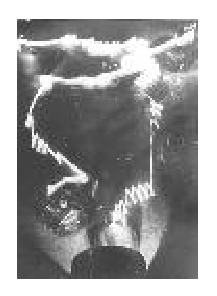
\includegraphics{notext_ps_logo}
   \end{tabular}
  &
  \hspace{5cm}
  &
  \begin{tabular}{r}
    {\bf USC Robotics Laboratory}\\
    University of Southern California\\
    Los Angeles, California, USA\\
  \end{tabular}
\end{tabular}
\vspace{5cm}
\centerline{\huge{Tclplayer}}
\vspace{0.5cm}
\centerline{\large{Version \VERSION\ Reference Manual}}
\vspace{2cm}

\centerline{\large Brian P. Gerkey}
\vspace{1cm}

\centerline{This document may not contain the most current documentation on}
\centerline{Tclplayer.  For the latest documentation, consult the Player 
homepage:}
\centerline{\HOMEPAGE}

\vspace{4cm}

\centerline{\today}

\newpage
\tableofcontents
\newpage

% reset page number to start with 1
\setcounter{page}{0}
\pagenumbering{arabic}
\section{Introduction}
Tclplayer is a Tcl package that provides procedures and data structures for
interacting with the Player robot device server.  Tclplayer has no special
requirements and should work with any recent ``vanilla'' version of Tcl.

Although Tcl is not an object-oriented language (and because {\tt [incr
Tcl]} is horrific), Tclplayer is built around the idea of an ``object'' that
holds information about your client's connection to the server.  Each of the
Tclplayer procedures takes as its first argument a variable that holds this
information.  This object is initialized by calling {\tt player\_connect}
(see Section~\ref{sect:player-connect}).  

Though the object is sometimes treated as an opaque structure, you will
often index into it directly (it is implemented as an array).  In general, you
can access device-specific data by referring to:
\begin{verbatim}
    $object($device,$index,$variable)
\end{verbatim}
where {\tt device} is the string name of the device, {\tt index} is the integer
index of the device, and {\tt variable} is the name of some device-specific
quantity of interest.  For convenience, data for the $0^{th}$ instance of 
each device (if it exists) is replicated without an index, e.g.:
\begin{verbatim}
    $object($device,$variable)
\end{verbatim}
Thus when accessing data from the $0^{th}$ instance of a device (a very
common thing to do), you may either use the index or leave it out.  In the
exposition on device details given below, we leave out the index for clarity.
Also, most Tclplayer procedures optionally take an index; if unspecified, the
index is assumed to be 0.

By the way, most of the Tclplayer procedures can throw Tcl errors.  This can
happen, for example, if a socket read fails.  If you want to handle these
errors yourself (instead of letting the program exit), you should {\tt catch} 
return values from Tclplayer procedures.

\section{Importing the code}
The Tcl client utilities are implemented as a standard Tcl package, named
Tclplayer.  In order to use it, you should set your {\tt TCLLIBPATH}
to include the directory above the directory in which the Tcl client code
resides.  For example, if you install Player in your home directory (as is
the default), you might do:
\begin{verbatim}
    $ export TCLLIBPATH=$TCLLIBPATH:$HOME/player-1.2/lib
\end{verbatim}
Then you can import the package in your own script as per normal:
\begin{verbatim}
    package require Tclplayer
\end{verbatim}
For this to work, however, there must be an appropriate {\tt pkgIndex.tcl} 
file as part of the Tclplayer package.  This will normally be built as part of
the Player build process.

\section{Generic functionality}
In this section we describe the device-neutral procedures provided by
Tclplayer.  Note that some procedures, notably {\tt player\_req} and {\tt
player\_write}, are not intended for user-level invocation, but rather should
be wrapped by device-specific procedures that provide friendlier interfaces.

\subsection{Connecting to the server}
\label{sect:player-connect}
In order to establish a connection to a Player server, you should call {\tt
player\_connect}:
\begin{verbatim}
    player_connect [-reqrep] obj [host] [port]
\end{verbatim}
Arguments are:
\begin{itemize}
\item {\tt [-reqrep]} : if specified, your connection will be placed into a
request / reply data mode
\item {\tt obj} : this variable will become the ``object'' that you will use
to control this connection
\item {\tt [host]} : if specified, a connection will be made to Player
listening on this host (default is {\tt "localhost"})
\item {\tt [port]} : if specified, a connection will be made to Player
listening on this port (default is {\tt \DEFAULTPORT})
\end{itemize}

\subsection{Disconnecting from the server}
To disconnect from the server, call {\tt player\_disconnect}, passing in the
connection-specific object:
\begin{verbatim}
    player_disconnect obj
\end{verbatim}

\subsection{Making requests}
An arbitrary configuration request may be made by calling {\tt player\_req}:
\begin{verbatim}
    player_req obj device index req
\end{verbatim}
Arguments are:
\begin{itemize}
\item {\tt obj} : the object for this connection
\item {\tt device} : the string name of the device to which the request is
made
\item {\tt index} : the integer index of the device to which the request is
made
\item {\tt req} : the (likely binary) string that is the request itself
\end{itemize}
This procedure will wait for the reply (discarding data received in the
meantime) and return the reply body.

\subsection{Requesting device access}
To simplify the common task of subscribing to (an unsubscribing from) devices,
a helper procedure {\tt player\_req\_dev} is provided:
\begin{verbatim}
    player_req_dev obj device access [index]
\end{verbatim}
Arguments are:
\begin{itemize}
\item {\tt device} : the string name of the device being accessed
\item {\tt access} : the requested access mode (should be {\tt r}, {\tt w},
{\tt a}, or {\tt c})
\item {\tt [index]} : if specified, the index of the device being accessed
(default is 0)
\end{itemize}
This procedure returns the access mode that was granted by the server ({\tt e}
indicates an error).

\subsection{Reading data}
To read one round of data (in a blocking fashion), call {\tt player\_read}:
\begin{verbatim}
    player_read obj
\end{verbatim}
Any new data will be stored in {\tt obj}.  Tclplayer keeps track of whether
your connection is continuous or request/reply, and {\tt player\_read} will
behave accordingly (e.g., by sending a request for data when necessary).

\subsection{Writing data}
To write a message to the server, call {\tt player\_write}:
\begin{verbatim}
    player_write obj device index str
\end{verbatim}
Arguments are:
\begin{itemize}
\item {\tt device} : the device for which the command is intended
\item {\tt index} : the index of said device
\item {\tt str} : the (likely binary) string that is the command itself
\end{itemize}

\subsection{Authentication}
If you are using Player's authentication facilities, then you can
request authentication for your client by calling {\tt player\_authenticate},
passing in the appropriate authentication key:
\begin{verbatim}
    player_authenticate obj key
\end{verbatim}

\section{The {\tt misc} device}
\subsection{Data}
Data from the {\tt misc} device is stored in 5 array entries:
\begin{itemize}
\item {\tt \$obj(misc,frontbumpers)} : the concatenated bitstring of the states
of the front bumpers
\item {\tt \$obj(misc,rearbumpers)} : the concatenated bitstring of the states
of the rear bumpers
\item {\tt \$obj(misc,battery)} : the battery potential (in volts)
\item {\tt \$obj(misc,analog)} : the value on the currently selected analog
input
\item {\tt \$obj(misc,digin)} : the concatenated bitstring of the digital
inputs
\end{itemize}

\section{The {\tt gripper} device}
\subsection{Data}
Data from the {\tt gripper} device is stored in 2 array entries:
\begin{itemize}
\item {\tt \$obj(gripper,byte0)} : the first byte of the gripper's state
\item {\tt \$obj(gripper,byte1)} : the second byte of the gripper's state
\end{itemize}

\section{The {\tt position} device}
\subsection{Data}
Data from the {\tt position} device is stored in 8 array entries:
\begin{itemize}
\item {\tt \$obj(position,xpos)} : $x$ coordinate of the odometric
position, where the $x$ axis is aligned with the robot's initial heading,
increasing forward (in mm)
\item {\tt \$obj(position,ypos)} : $y$ coordinate of the odometric
position, where the $y$ axis is orthogonal to the robot's initial heading,
increasing leftward (in mm)
\item {\tt \$obj(position,heading)} : odometric heading (in
degrees)
\item {\tt \$obj(position,speed)} : current translational velocity (in
mm/sec)
\item {\tt \$obj(position,sidespeed)} : current sideways velocity (in
mm/sec); only used with holonomic robots
\item {\tt \$obj(position,turnrate)} : current angular velocity (in
degrees/sec)
\item {\tt \$obj(position,compass)} : current compass heading (in degrees)
\item {\tt \$obj(position,stall)} : concatenated bitstring of left and right
motor stall sensors
\end{itemize}

\subsection{Command}
New position commands are sent by calling {\tt player\_set\_speed}:
\begin{verbatim}
    player_set_speed obj fv tv [index]
\end{verbatim}
where {\tt fv} and {\tt tv} are forward and turn velocities, respectively.

For convenience, you can stop the robot (i.e., command zero velocities)
by the calling:
\begin{verbatim}
    player_stop_robot obj
\end{verbatim}

\subsection{Configuration}
The motors cay be turned on and off by calling:
\begin{verbatim}
    player_change_motor_state obj state [index]
\end{verbatim}
where non-zero {\tt state} will enable the motors, and zero will disable them.

\section{The {\tt sonar} device}
\subsection{Data}
Data from the {\tt sonar} device is stored in $n$ array 
entries, where each entry is a range reading from a separate transducer:
\begin{itemize}
\item {\tt \$obj(sonar,count)} : the number of range readings
\item {\tt \$obj(sonar,\$i)} : the $i^{th}$ sonar's range (in mm)
\end{itemize}

\subsection{Configuration}
The sonars cay be turned on and off by calling:
\begin{verbatim}
    player_change_sonar_state obj state [index]
\end{verbatim}
where non-zero {\tt state} will enable the motors, and zero will disable them.

\section{The {\tt laser} device}
\subsection{Data}
Meta-data from the {\tt laser} device is stored in 4 array entries:
\begin{itemize}
\item {\tt \$obj(laser,min\_angle)} : the starting angle of the scan (in
hundredths of a degree)
\item {\tt \$obj(laser,max\_angle)} : the ending angle of the scan (in
hundredths of a degree)
\item {\tt \$obj(laser,resolution)} : the angular resolution of the scan (in
hundredths of a degree)
\item {\tt \$obj(laser,range\_count)} : the number of range readings included
in the scan
\end{itemize}
The range readings themselves are stored in $n$ array entries:
\begin{itemize}
\item {\tt \$obj(laser,\$i)} : the $i^{th}$ range reading (in mm)
\end{itemize}

\subsection{Configuration}
The {\tt laser} device can be configured by calling {\tt
player\_config\_laser}:
\begin{verbatim}
    player_config_laser obj min_angle max_angle \
                        resolution intensity [index]
\end{verbatim}
where the arguments have the same meaning as they do in the data, as described
in the previous section.

\section{The {\tt vision} device}
\subsection{Data}
Because virtually any number of colored blobs can be found in the camera image 
at a given moment, the {\tt vision} device produces variable-length data,
which is organized by color channel.  The data for channel $i$ (where 
$i \in [0,31]$) are stored as follows:
\begin{itemize}
\item {\tt \$obj(vision,\$i,numblobs)} : the number of blobs detected on
channel $i$
\item {\tt \$obj(vision,\$i,\$j,color)} : the color of the $j^{th}$ blob on
channel $i$ (as a Tk-format 6-digit hexadecimal color string: \#RRGGBB)
\item {\tt \$obj(vision,\$i,\$j,area)} : the area of the $j^{th}$ blob on
channel $i$ (in pixels)
\item {\tt \$obj(vision,\$i,\$j,x)} : the $x$ coordinate of the center of the 
$j^{th}$ blob on channel $i$ (in pixels)
\item {\tt \$obj(vision,\$i,\$j,y)} : the $y$ coordinate of the center of the 
$j^{th}$ blob on channel $i$ (in pixels)
\item {\tt \$obj(vision,\$i,\$j,left)} : the left boundary of the $j^{th}$ 
blob on channel $i$ (in pixels)
\item {\tt \$obj(vision,\$i,\$j,right)} : the right boundary of the $j^{th}$ 
blob on channel $i$ (in pixels)
\item {\tt \$obj(vision,\$i,\$j,top)} : the top boundary of the $j^{th}$ 
blob on channel $i$ (in pixels)
\item {\tt \$obj(vision,\$i,\$j,bottom)} : the bottom boundary of the $j^{th}$ 
blob on channel $i$ (in pixels)
\end{itemize}

\section{The {\tt ptz} device}
\subsection{Data}
Data for the {\tt ptz} device (a pan-tilt-zoom camera unit) is stored in 
3 array entries:
\begin{itemize}
\item {\tt \$obj(ptz,pan)} : the pan angle of the camera, increasing
counterclockwise with 0 being forward (in degrees)
\item {\tt \$obj(ptz,tilt)} : the tilt angle of the camera, increasing upward
with 0 being level (in degrees)
\item {\tt \$obj(ptz,zoom)} : the zoom of the camera, increasing with greater
zoom (0 is wide; 1023 is telefoto)
\end{itemize}

\subsection{Command}
New commands are sent to the {\tt ptz} device by calling {\tt
player\_set\_camera}:
\begin{verbatim}
    player_set_camera obj p t z [index]
\end{verbatim}
where {\tt p}, {\tt t}, and {\tt z} are new pan, tilt, and zoom values,
respectively.

\section{The {\tt audio} device}
This device is not supported.

\section{The {\tt laserbeacon} device}
\subsection{Data}
This device can return a variable number of beacons:
\begin{itemize}
\item {\tt \$obj(laserbeacon,numbeacons)} : the number of detected beacons
\end{itemize}
The data concerning the $i^{th}$ detected beacon is stored in 4 array entries:
\begin{itemize}
\item {\tt \$obj(laserbeacon,\$i,id)} : the integer ID of the beacon, or 0 if 
the signature could not be decoded
\item {\tt \$obj(laserbeacon,\$i,range)} : the range to the beacon from the
laser (in mm)
\item {\tt \$obj(laserbeacon,\$i,bearing)} : the bearing to the beacon
relative to the laser (in degrees)
\item {\tt \$obj(laserbeacon,\$i,orient)} : the orientation of the beacon
relative to the laser (in degrees)
\end{itemize}

\subsection{Configuration}
You can set the current {\tt laserbeacon} configuration:
\begin{verbatim}
    player_config_laserbeacon obj bit_count bit_size zero_thresh \
                              one_thresh [index]
\end{verbatim}

\section{The {\tt broadcast} device}
This device is not supported.

\section{The {\tt speech} device}
This device is not supported.

\section{The {\tt gps} device}
The data for the {\tt gps} device is store in 3 array entries:
\begin{itemize}
\item {\tt \$obj(gps,x)} : the $x$ coordinate of the current pose (in mm)
\item {\tt \$obj(gps,y)} : the $y$ coordinate of the current pose (in mm)
\item {\tt \$obj(gps,heading)} : the $\theta$ coordinate of the current pose 
(in degrees)
\end{itemize}

\section{The {\tt bps} device}
This device is not supported.

\end{document}
